%-----------------------------------------------------------------------------%
\chapter{\babEmpat}
\label{bab:4}
%-----------------------------------------------------------------------------%

In this chapter, we present the results from our experiments.

%-----------------------------------------------------------------------------%
\section{Experimental Setup}
\label{sec:experimentalSetup}
%-----------------------------------------------------------------------------%

This section details the experimental setup.

%-----------------------------------------------------------------------------%
\subsection{Dataset}
\label{sec:dataset-experiment}
%-----------------------------------------------------------------------------%
In this experiment, we utilize the ExplainEthics dataset developed by Quan et al. \citep{quan2024enhancing} which is built upon the ETHICS dataset developed by Hendrycks et al. \citep{hendrycks2020aligning}. The dataset utilized in our pipeline consists of a total of 145 data points, broken down into six specific moral norm violations: \texttt{violate\_care} (74 cases), \texttt{violate\_authority} (27 cases), \texttt{violate\_fairness} (21 cases), \texttt{violate\_sanctity} (19 cases), \texttt{violate\_liberty} (2 cases), and \texttt{violate\_loyalty} (2 cases). Each data point presents a moral scenario that violates one of these moral foundations. 

For example, a problem instance includes the context: ``\textit{I covered up the truth about their employee spreading fake news.}'' alongside an explanation of the underlying ethical reasoning: ``\textit{covering up the truth about an employee spreading fake news is a form of deception. harm to the reputation of a group, especially a company, can be seen as a behavior involving cheating and deception. deception is a form of dishonest behavior which can harm the reputation of a group, in this case, the company. spreading fake news is a form of deception and dishonesty.}'' The pipeline's objective is to deduce the target query, denoted as the \texttt{gold\_foundation}, which in this example is \texttt{violate\_fairness}. The system evaluates the natural language premises against this target to formally establish whether the scenario entails the specified moral violation.

%-----------------------------------------------------------------------------%
\subsection{Models, Solvers, and Baselines}
\label{sec:modelsAndBaselines}
%-----------------------------------------------------------------------------%
% Llama-3.1-8B-Instruct, Mistral-7B, Qwen-7B, etc.
To provide a clearer overview of the language models employed across the different stages of the ARGOS algorithm, Table~\ref{tab:models_usage} maps each specific algorithmic subroutine to its corresponding model along with the generation configuration. For the declarative prompting phase, where we translate the query and initial explanation from natural language to formal logic representations \citep{ye2023satlm}, we utilize the Qwen/Qwen2.5-Coder-7B-Instruct model. In our main experiment for the abductive reasoning steps, we utilize the Llama-3.1-8B-Instruct model. This includes the neural fallback mechanism, the generation of candidate commonsense rules, and the two independent neural filtering gates. To evaluate the impact of the language models on the generated commonsense premises, we also swap the main reasoning model with Qwen/Qwen2.5-7B-Instruct and Mistral-7B-Instruct in the ablation study (Section~\ref{sec:impactOfLanguageModel}).

\begin{table}[H]
    \centering
    \caption{Mapping of algorithmic subroutines to the utilized language models and their generation configuration in the main experiment.}
    \label{tab:models_usage}
    \begin{tabular}{lp{3cm}p{4.5cm}p{3cm}}
        \toprule
        \textbf{Algorithm Term} & \textbf{Algorithmic Task} & \textbf{Assigned Model} & \textbf{Configuration} \\
        \midrule
        N/A & Declarative Prompting & Qwen/Qwen2.5-Coder-7B-Instruct & Greedy ($T=0$), 4-bit NF4 \\
        \texttt{llm\_solve} & Neural CoT Fallback & Llama-3.1-8B-Instruct$^\dagger$ & Greedy ($T=1$, \texttt{top\_k}=0), 4-bit NF4 \\
        \texttt{llm\_confidence} & CoT Confidence Scoring & Llama-3.1-8B-Instruct$^\dagger$ & Log-prob scoring, 4-bit NF4 \\
        \texttt{find\_new\_commonsense} & Commonsense Generation & Llama-3.1-8B-Instruct$^\dagger$ & Greedy ($T=1$, \texttt{top\_k}=0), 4-bit NF4 \\
        \texttt{commonsense\_score} & Commonsense Validity & Llama-3.1-8B-Instruct$^\dagger$ & Log-prob scoring, 4-bit NF4 \\
        \texttt{relevance\_score} & Relevance Check & Llama-3.1-8B-Instruct$^\dagger$ & Log-prob scoring, 4-bit NF4 \\
        \midrule
        \multicolumn{4}{l}{$^\dagger$\textit{Also evaluated with: Qwen/Qwen2.5-7B-Instruct and Mistral-7B-Instruct (see Section~\ref{sec:impactOfLanguageModel})}} \\
        \bottomrule
    \end{tabular}
\end{table}

All models are loaded in 4-bit NF4 quantization using the BitsAndBytes library with double quantization enabled and bfloat16 compute dtype. The \textit{generative} tasks (\texttt{llm\_solve} and \texttt{llm\_generate}) use greedy decoding, as the \texttt{temperature} parameter is set to $T=1$ but \texttt{top\_k} is set to 0, which bypasses stochastic sampling (the condition \texttt{do\_sample = (T > 0 and top\_k > 0)} evaluates to \texttt{False}). The \textit{scoring} tasks (\texttt{llm\_confidence}, \texttt{llm\_commonsense\_score}, and \texttt{llm\_relevance\_score}) do not generate text, but instead compute log-probabilities over fixed answer tokens (e.g., ``Yes'' vs.\ ``No'') to produce a confidence score.

In our experiment, we utilize CaDiCaL 2.0 \citep{biere2024cadical} as the SAT solver to determine whether a norm query is satisfiable and CadiBack \citep{biere2023cadiback} for extracting our backbones.

To evaluate the impact of the proposed approach, Chain-of-Thought (CoT) prompting is used as the baseline, as it represents a standard method for eliciting simulated reasoning in language models.



%-----------------------------------------------------------------------------%
\subsection{ARGOS Pipeline Configuration}
\label{sec:argosConfig}
%-----------------------------------------------------------------------------%
% - rule_thresh=0.3, cot_thresh=0.8, annealing schedule
% - Number of SC samples per iteration (n=5)
The commonsense threshold $\tau \in \{0.3, 0.5, 0.8\}$ is evaluated to determine its efficacy in filtering illogical premises. We use an LLM confidence threshold of $\gamma = 0.8$ as the default configuration for the main experiments. Additionally, we test an LLM confidence threshold of $\gamma = 1.3$ to analyze the pipeline's behavior when the SAT solver is forced to attempt query resolution independently, without relying on an early neural fallback. Since the confidence score generated by the language model is mathematically bounded by a maximum of 1.0, setting $\gamma = 1.3$ ensures that the LLM will never reach the required confidence to trigger an early decision, effectively bypassing the early exit mechanism entirely.


%-----------------------------------------------------------------------------%
\section{Overall Accuracy Results}
\label{sec:overallAccuracy}
%-----------------------------------------------------------------------------%
% → answers RQ3


%-----------------------------------------------------------------------------%
\subsection{ARGOS vs CoT Baseline}
\label{sec:argosVsBaselines}
%-----------------------------------------------------------------------------%

The overall performance comparison of ARGOS across different rule thresholds ($\tau$) against the CoT Baseline is presented in Table~\ref{tab:overall_results}.

\begin{table}[ht]
    \centering
    \caption{Overall performance comparison of ARGOS across different rule thresholds ($\tau$) against the CoT Baseline}
    \label{tab:overall_results}
    \begin{tabular}{lcccc}
        \toprule
        \textbf{Model Configuration} & \textbf{Accuracy} & \textbf{Precision} & \textbf{Recall} & \textbf{F1 Score} \\
        \midrule
        CoT Baseline (SC) & 0.275 & 0.116 & 0.120 & 0.111 \\
        ARGOS ($\tau \in \{0.3, 0.5, 0.8\}$) & 0.609 & 1.000 & 0.686 & 0.803 \\
        \bottomrule
    \end{tabular}
\end{table}

Table~\ref{tab:overall_results} shows the performance of the ARGOS pipeline and the baseline Chain-of-Thought (CoT) prompting. This CoT with Self-Consistency experiment was conducted using the \texttt{meta-llama/Llama-3.1-8B-Instruct} model and a standalone 4-shot prompt that appended ``Let's think step by step'' to elicit intermediate reasoning (the complete CoT prompt is detailed in Appendix~\ref{appendix:prompts}). The model independently generated 3 reasoning paths (3-shot self-consistency), selecting the final predicted norm via a majority vote. Under this setup, the baseline model achieves an average accuracy of 0.275. In contrast, the ARGOS neurosymbolic pipeline achieves an accuracy of 0.609 on the 128 queries requiring abductive reasoning.

The pipeline was evaluated across three rule confidence thresholds ($\tau \in \{0.3, 0.5, 0.8\}$). The overall accuracy remains constant at 0.609 across all evaluated thresholds. Therefore, Table~\ref{tab:overall_results} specifically highlights the results for $\tau=0.3$, which represents the highest leniency in accepting candidate rules. To prevent artificially inflating these results, we separately evaluated 10 queries that were immediately solved by the SAT solver without triggering the commonsense clause generation process. These instances occurred because the natural language translation of their premises already contained the target query. Formally, if the set of premises is $\mathcal{P} = \{P_1, P_2, \dots, P_n\}$ and the query $Q$ is already present in this set ($Q \in \mathcal{P}$), the conjunction trivially entails the query: $(P_1 \land P_2 \land \dots \land P_n \land Q) \vdash Q$.


%-----------------------------------------------------------------------------%
\subsection{Per-Norm Accuracy Breakdown}
\label{sec:perNormAccuracy}
%-----------------------------------------------------------------------------%
Figure~\ref{fig:per_norm_acc} shows the accuracy breakdown per gold standard norm for the $\tau=0.3$ configuration.

\begin{figure}[H]
    \centering
    
\includegraphics[width=0.8\textwidth]{assets/explainethics_per_norm_acc.png}
    \caption{Per-norm accuracy of ARGOS ($\tau \in \{0.3, 0.5, 0.8\}$) on the ExplainEthics dataset.}
    \label{fig:per_norm_acc}
\end{figure}

Table~\ref{tab:argos_per_norm_comparison} details the specific distribution of True Positives (TP), False Negatives (FN), True Negatives (TN), and False Positives (FP) for each moral norm.

\begin{table}[H]
    \centering
    \caption{Per-norm accuracy and confusion matrix breakdown for ARGOS ($\tau \in \{0.3, 0.5, 0.8\}$)}
    \label{tab:argos_per_norm_comparison}
    \begin{tabular}{lccccc}
        \toprule
        \textbf{Norm} & \textbf{Accuracy} & \textbf{TP} & \textbf{FN} & \textbf{TN} & \textbf{FP} \\
        \midrule
        Violate Authority & 0.680 & 17 & 8 & 113 & 0 \\
        Violate Care      & 0.528 & 38 & 34 & 66 & 0 \\
        Violate Fairness  & 0.722 & 13 & 5 & 120 & 0 \\
        Violate Liberty   & 1.000 & 2 & 0 & 136 & 0 \\
        Violate Loyalty   & 0.500 & 1 & 1 & 136 & 0 \\
        Violate Sanctity  & 0.684 & 13 & 6 & 119 & 0 \\
        \bottomrule
    \end{tabular}
\end{table}

As detailed in Table~\ref{tab:argos_per_norm_comparison}, the accuracy on the \textit{Liberty} and \textit{Sanctity} norms is 1.000 and 0.684 respectively. The accuracy on the \textit{Care} norm is 0.528. The accuracy on the \textit{Authority} and \textit{Fairness} norms is 0.680 and 0.722, respectively. The accuracy on the \textit{Loyalty} norm is 0.500. The ARGOS pipeline records a Precision of 1.000, which corresponds to zero False Positives ($FP = 0$). This occurs because the evaluated subset of the ExplainEthics dataset consists exclusively of scenarios where a norm is actually violated (i.e., there are no ground-truth negative examples labeled as ``does not violate''). Consequently, when the model predicts a violation, its prediction is either a True Positive (it correctly identifies the violated norm) or a False Negative for the target norm (it predicts a norm other than the ground truth). Because there are no genuine negative instances, it is impossible for the pipeline to generate a False Positive, fixing $FP$ to zero and artificially inflating Precision to its maximum value.




%-----------------------------------------------------------------------------%
\section{SAT Solver Utilization}
\label{sec:satSolverUtilization}
%-----------------------------------------------------------------------------%
% → answers RQ2


%-----------------------------------------------------------------------------%
\subsection{Resolution Pathways Distribution}
\label{sec:distributionOfPathways}
%-----------------------------------------------------------------------------%
To understand the efficacy of each component in the neurosymbolic pipeline, we categorize the evaluation results into distinct ``resolution pathways''. A resolution pathway describes the specific stage in the ARGOS algorithm where a query successfully reaches a final conclusion or ultimately fails. The queries are classified into three possible pathways: (1) \textit{pre-solved by SAT}, where the initial natural language translation is sufficient for formal entailment without abductive generation since the natural language translation already includes the query among the premises, as stated in Section~\ref{sec:argosVsBaselines}; (2) \textit{resolved by the backbone loop}, where the SAT solver successfully deduces the answer after iteratively acquiring new commonsense rules; or (3) \textit{resolved by the neural CoT fallback}, where the symbolic engine fails to find a proof and the system relies entirely on the language model's internal Chain-of-Thought reasoning to reach a final decision (whether correct or incorrect).

\begin{figure}[H]
    \centering
    
\includegraphics[width=0.6\textwidth]{assets/explainethics_resolution_pie.png}
    \caption{Distribution of solving methods for ARGOS ($\tau=0.5$).}
    \label{fig:resolution_pie}
\end{figure}

Figure~\ref{fig:resolution_pie} shows this distribution. Out of the 138 total queries evaluated in the pipeline, exactly 10 queries (7.2\%) were pre-solved by the SAT solver through formal entailment via the initial CNF translation, achieving an accuracy of 1.000 (10/10). The remaining 128 queries entered the abductive generation loop. However, none of these queries (0\%) were successfully resolved by the backbone loop itself due to the LLM's inability to navigate the vast propositional search space and generate clauses that converge toward the target query. Consequently, these 128 queries bypassed the backbone and were pushed to the third pathway, relying entirely on the neural Chain-of-Thought (CoT) fallback mechanism. Of these 128 CoT-resolved queries, 84 queries (65.6\%) were answered correctly, while the remaining 44 queries (34.4\%) were answered incorrectly.





%-----------------------------------------------------------------------------%
\subsection{Analysis of Symbolic Resolution}
\label{sec:backboneConvergence}
%-----------------------------------------------------------------------------%
As detailed in Section~\ref{sec:argosVsBaselines}, the 10 queries that were formally resolved by SAT were all pre-solved by the initial CNF. This occurred because the natural language translation of their premises inadvertently contained the target query, allowing the SAT solver to trivially deduce the answer immediately without executing the iterative ARGOS loop. Because this success is due to the natural language translation already including the query in the premises, the evaluation of the ARGOS loop itself is completely separated from these pre-solved instances in the overall metrics. 

For the remaining 128 queries, the neurosymbolic pipeline failed to reach a formal symbolic resolution. Rather than narrowing down toward a definitive proof, the iterative commonsense generation process continuously adds new literals to the backbone. Because the domain of moral reasoning relies heavily on propositional logic without explicit entity constraints, the search space inflates exponentially. Consequently, the backbone expands indefinitely without successfully deducing the target query, forcing all 128 of these unresolved queries to ultimately rely on the neural fallback mechanism.

%-----------------------------------------------------------------------------%
% \section{Comparison with CLUTRR and ProntoQA}
% \label{sec:comparisonWithClutrrAndPronto}
% %-----------------------------------------------------------------------------%
% % → answers RQ1


% %-----------------------------------------------------------------------------%
% \subsection{Entailment Success Rate}
% \label{sec:entailmentSuccessRate}
% %-----------------------------------------------------------------------------%
% % % of datapoints where SAT solver achieved UNSAT (= formal proof)
% % across the three datasets

%-----------------------------------------------------------------------------%
\section{Ablation Study: Disabling Early CoT Exit}
\label{sec:ablationStudy}
%-----------------------------------------------------------------------------%
To analyze the impact of the neural fallback threshold, an ablation study was conducted using the \texttt{meta-llama/Llama-3.1-8B-Instruct} model with an initial neural fallback configuration of $\gamma = 1.3$. We initially sampled the first 20 data points for this ablation study for simplicity. However, 2 out of these 20 queries were pre-solved directly by the SAT solver because their translated premises inadvertently contained the target query, leaving an active 18-example ablation subset. Because the confidence score of the language model can never exceed 1.0, this starting configuration effectively disables the early CoT exit mechanism, forcing the pipeline to engage in abductive premise generation iterations. 

On this 18-example ablation subset, the pipeline achieved an overall accuracy of 50.0\%, outperforming the baseline Chain-of-Thought (CoT) prompting with Self-Consistency, which only achieved 33.3\% accuracy. The baseline CoT with Self-Consistency experiment was conducted by utilizing a standalone 3-shot prompt that appended ``Let's think step by step'' to elicit intermediate reasoning. The model then independently generated 20 reasoning paths, with the final predicted norm selected via a majority vote. As we can see in Figure~\ref{fig:ablation_resolution_pie}, it is important to note that the 50.0\% accuracy achieved by ARGOS was not achieved formally by the SAT solver reaching an entailment after commonsense clause generation. Instead, this accuracy was achieved entirely through the neural CoT fallback after the confidence threshold $\gamma$ was gradually decremented by $\alpha=0.1$ during each unsuccessful generation iteration, eventually allowing the LLM's fallback answer to pass.

\begin{figure}[H]
    \centering
    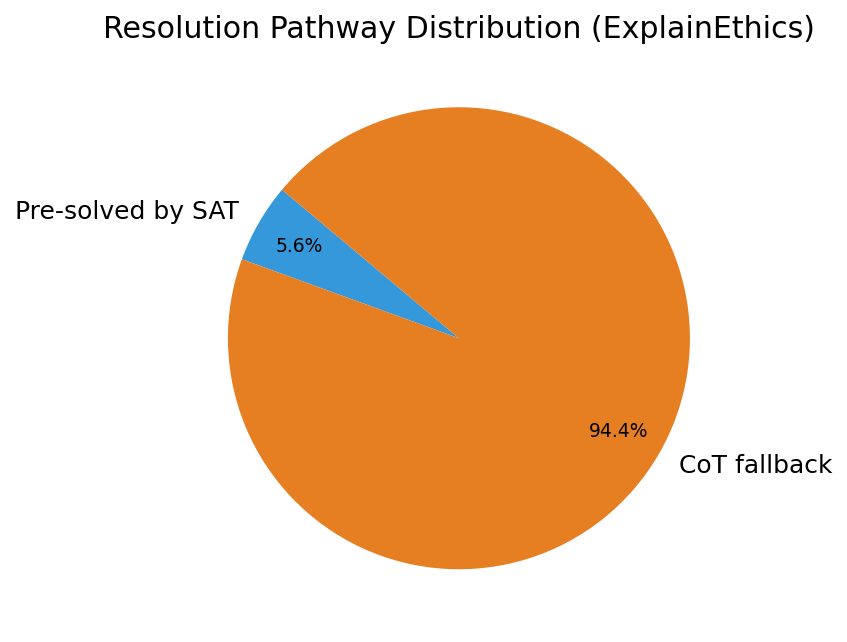
\includegraphics[width=0.6\textwidth]{assets/ablation_1.3/explainethics_resolution_pie.png}
    \caption{Distribution of resolution pathways with early CoT exit disabled ($\gamma=1.3$).}
    \label{fig:ablation_resolution_pie}
\end{figure}

Figure~\ref{fig:ablation_resolution_pie} shows the resolution pathway distribution for this ablation configuration. 

\begin{figure}[H]
    \centering
    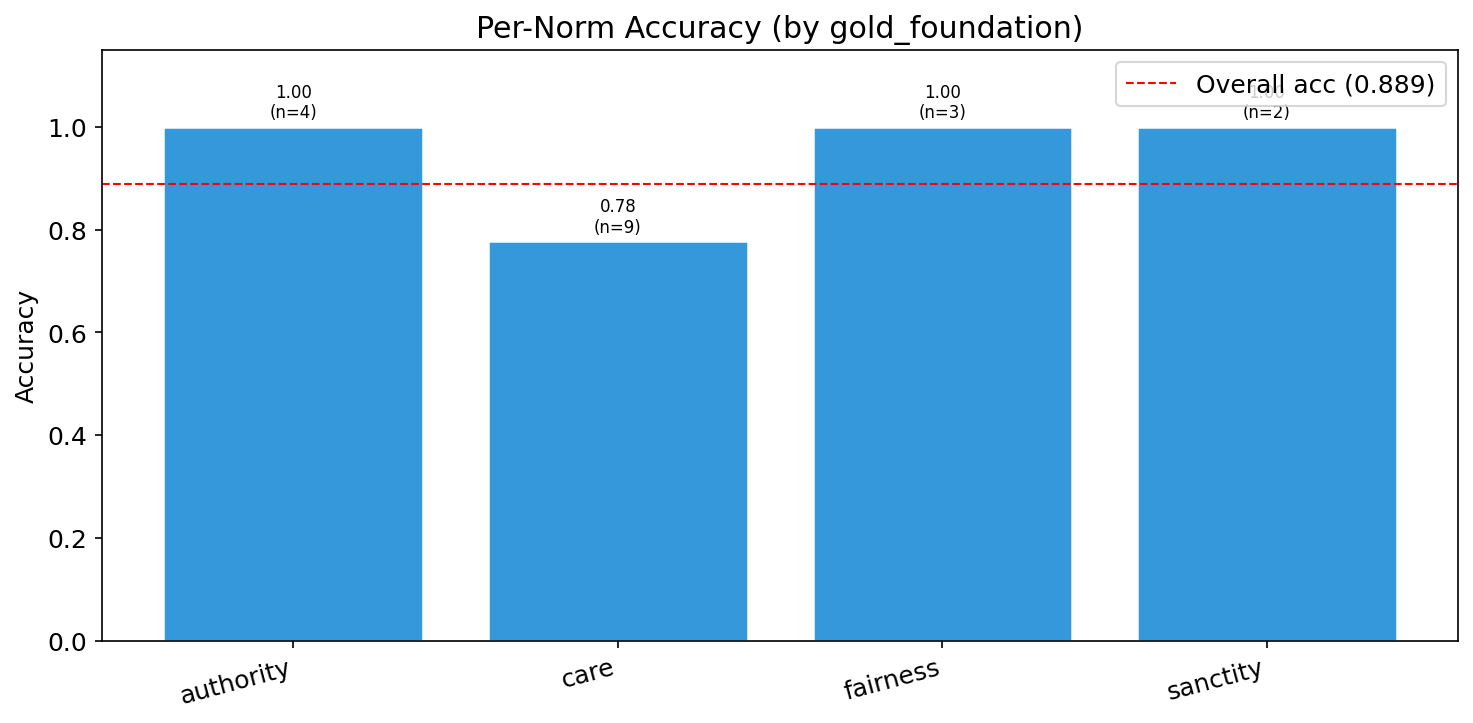
\includegraphics[width=0.8\textwidth]{assets/ablation_1.3/explainethics_per_norm_acc.png}
    \caption{Per-norm accuracy of the ablation study ($\gamma=1.3$).}
    \label{fig:ablation_per_norm_acc}
\end{figure}

Figure~\ref{fig:ablation_per_norm_acc} shows the accuracy breakdown per norm for the ablation study. Note that any moral norm that does not appear in this figure was not included in the 20 initially sampled data points.

The pipeline achieved varying degrees of accuracy across different norms depending on the specific predictions made during the CoT fallback.

%-----------------------------------------------------------------------------%
\section{Impact of Language Model}
\label{sec:impactOfLanguageModel}
%-----------------------------------------------------------------------------%
To evaluate the impact of the underlying language model on the pipeline's reasoning capabilities, we conducted an experiment comparing the Llama-3.1-8B-Instruct, Qwen/Qwen2.5-7B-Instruct, and Mistral-7B-Instruct models for the \texttt{find\_new\_commonsense}, \texttt{commonsense\_score}, and \texttt{relevance\_score} subroutines. A detailed qualitative analysis of how these models differ in their generated commonsense clauses is presented in Section~\ref{sec:subjectiveBeliefs}. 

To ensure that the models exhaust the generation loops and expose their distinct commonsense rules rather than relying on early answers, we evaluated them on the same 18-example ablation subset as used in Section~\ref{sec:ablationStudy}, with the early CoT exit threshold disabled ($\gamma=1.3$). The results of this evaluation are summarized in Table~\ref{tab:model_per_norm_comparison}.

Table~\ref{tab:model_per_norm_comparison} details the breakdown of accuracy and prediction rates (TP, FN, TN, FP) per moral norm. The Qwen/Qwen2.5-7B-Instruct model achieved the highest performance with an overall accuracy of 61.1\%, notably performing well on the \textit{Authority} (0.750) and \textit{Care} (0.444) norms. The Llama-3.1-8B-Instruct model achieved 50.0\% overall accuracy, and the Mistral-7B-Instruct model achieved 44.4\% accuracy. Despite the varying degrees of success across different norms, all three models outperformed the CoT Self-Consistency baseline (which achieved 33.3\% overall accuracy on this subset), demonstrating that the neurosymbolic ARGOS pipeline consistently enhances the reasoning capabilities of different language models by leveraging their internal commonsense clauses.

\begin{table}[H]
    \centering
    \caption{Per-norm accuracy and confusion matrix breakdown across different language models on the ablation subset ($\gamma=1.3$)}
    \label{tab:model_per_norm_comparison}
    \begin{tabular}{llccccc}
        \toprule
        \textbf{Model} & \textbf{Norm} & \textbf{Accuracy} & \textbf{TP} & \textbf{FN} & \textbf{TN} & \textbf{FP} \\
        \midrule
        Llama-3.1-8B-Instruct 
        & Violate Authority & 0.500 & 2 & 2 & 14 & 0 \\
        & Violate Care      & 0.333 & 3 & 6 & 9  & 0 \\
        & Violate Fairness  & 1.000 & 3 & 0 & 15 & 0 \\
        & Violate Sanctity  & 0.500 & 1 & 1 & 16 & 0 \\
        \midrule
        Mistral-7B-Instruct 
        & Violate Authority & 0.250 & 1 & 3 & 14 & 0 \\
        & Violate Care      & 0.333 & 3 & 6 & 9  & 0 \\
        & Violate Fairness  & 1.000 & 3 & 0 & 15 & 0 \\
        & Violate Sanctity  & 0.500 & 1 & 1 & 16 & 0 \\
        \midrule
        Qwen/Qwen2.5-7B-Instruct 
        & Violate Authority & 0.750 & 3 & 1 & 14 & 0 \\
        & Violate Care      & 0.444 & 4 & 5 & 9  & 0 \\
        & Violate Fairness  & 1.000 & 3 & 0 & 15 & 0 \\
        & Violate Sanctity  & 0.500 & 1 & 1 & 16 & 0 \\
        \bottomrule
    \end{tabular}
\end{table}
